\chapter{Working with the Data Explorer}

\section{Loading data...}

\subsection{Native File Formats}

\ogs has a large number of native file formats for storing geometrical data (*.gli), meshes (*.msh), processes (*.pcs), FEM conditions (such as boundary conditions (*.bc)) and material properties (e.g. fluid properties (*.mfp)) and many more.

Not all of them can be loaded into the user interface since not all of them contain data that can be visualised. Things are additionally made difficult as the file standards for the programm are currently changed to XML files\footnote{http://www.w3.org/XML/}. For this reason there exists -- at least at the time of this writing -- two file standards for certain kinds of objects. Hopefully, this unfortunate situation is resolved soon.

You can open native OGS files by clicking \cmd{File\ra Open...}. Supported native \ogs formats are:
\begin{itemize}
\item Geometrical data files (*.gli)\\
    Containing geometrical data such as points, polylines and surfaces (in this file format surfaces are defined by closed polylines and are therefore always describing planes).
\item Geometrical XML data files (*.gml)\\
    Containing geometrical data such as points, polylines and surfaces (in this file format surfaces are triangulated and can therefore describe any kind of surface).
\item Observation sites (*.stn)\\
    XML file format containing information for observation stations as well as boreholes. The files also describe points in space but with additional information (such as stratigraphic information for boreholes). Also, this data is visualised in a different way.
\item Mesh files (*.msh) containing structured or unstructured grids.
\item FEM conditions (*.bc, *.ic, *.st)\\
    Describing inital- and boundary conditions as well as source terms as special geometrical objects (points, polylines, surfaces) with additional information important for a subsequent simulation.
\item FEM conditions (*.cnd)
    XML file format of the previous kind of data.
\end{itemize}

\subsection{Import File Formats}

\begin{figure}[tb]
\begin{center}
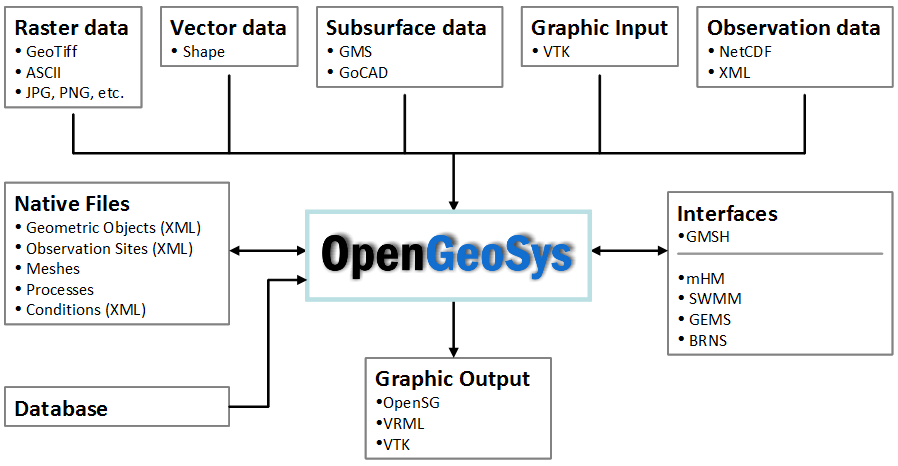
\includegraphics[width=0.99\linewidth]{interfaces}
\caption{Supported file formats for import and export of data.}
\label{fig:interfaces}
\end{center}
\end{figure}

A number of non-native file formats can also be loaded and visualised in the Data Explorer. To import these files click on \cmd{File \ra Import Files} and select the appropriate entry.

Depending of which file format you want to load, quality of the interface varies depending on a number of facts such as if the file format is an open standard or if there were enough input files to test the interface when it was implemented.

Currently the following file formats are supported:
\begin{itemize}
\item ESRI \textbf{shape} files (*.shp)\\
Vector files specifying points, polylines and polygons. The interface for shape files is thoroughly tested and there should be no problems whatsoever. However, note that a lot shape files come with a database file containing additional information (*.dbf) which has no standardised table structure and therefore is not analysed or imported by the data explorer.
\item Aquaveo \textbf{GMS} files (*.txt, *.3dm)\\
Text or mesh files specifying boreholes (*.txt) or layered meshes build from tetrahedrons and prisms. This interface has been tested with number of cases and should work fine.
\item \textbf{GMSH} files (*.msh)\\
Mesh files containing unstructured grids. As an exception these files are \emph{not} loaded via the import menu but you have to load them directly via \cmd{File\ra Open...}. The interface should work perfectly however.
\item \textbf{GoCAD} files (*.ts)\\
This interface is in an unfinished state. However, there exists a programming interface to write OGS-files directly from GoCAD. Please talk to the development team if you need to load data into OGS.
\item \textbf{NetCDF} files (*.nc, *.cdf)\\
A machine-independent format that contains all kinds array-oriented scientific data. This interface works only under certain circumstances and you should probably talk to the development team if you want to load netCDF files into OGS.
\item \textbf{Petrel} files\\
This interface is in an unfinished state. Please talk to the development team if you need to load data into OGS.
\item \textbf{Raster} files (*.asc, *.bmp, *.jpg, *.png, *.tif)\\
Image data files that may contain satellite images, etc. Ascii raster files (*.asc) and GeoTIFF (*.tif) files contain geo-referenced data, while common image files (*.bmp, *.jpg, *.png) do not. This interface should work perfectly although it can be quite slow for large raster files.
\item Visual Toolkit (\textbf{VTK}) files (*.vti, *.vtk, *.vtp, *.vtr, *.vts, *.vtu)\\
Files containing data for graphic objects, ranging from image files (*.vti) to structured (*.vts) or unstructured meshes (*.vtu). All data sets may include additional data in the form of scalar arrays. This interface should work perfectly.
\end{itemize}

\subsection{Removal of Data}

You can remove all data loaded into \ogs by right-clicking the data set in its respective data view and selected \cmd{Remove data}. Specifically you can also remove only polylines or surfaces only from a geometry. The only exception to this rule are geometric points which can only be removed if both surfaces and polylines are already deleted as both kinds of objects are dependent on points. Regardless of the previous remarks you can also remove geometries as whole.

\section{Data Visualisation}
\label{datavisualisation}

Technically, data (or a representation thereof) loaded into the programme is displayed at three different locations (see figure \ref{fig:gui}):

\subsection{Data Views}

There are four different DataView-Tabs in the programme where the data is visible in the form of lists. Which of the tabs is used depends on the data. There is one tab for geometrical information, one for meshes, one for stations (i.e. observation sites) and one for FEM conditions (i.e. boundary conditions, etc.)

The DataView for geometrical information contains a list of geometries. Each geometry-item has up to three children titled ``Points'', ``Polylines'' and ``Surfaces'' containing the information about the respective geometrical objects. For example, the item `Points' contains a list of points and for each item (i.e. each point) its index, the coordinates and (if existing) the name of the object can be displayed. Each geometry \emph{needs} to contain a list of points. Other geometrical objects (i.e. polylines or surfaces) are optional.

\subsection{Render Window}

\begin{figure}[tb]
\begin{center}
\subfloat{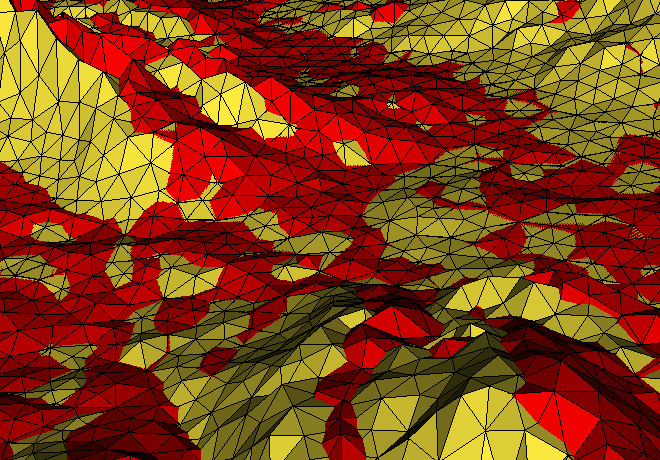
\includegraphics[width=0.48\linewidth]{error1}}\enspace
\subfloat{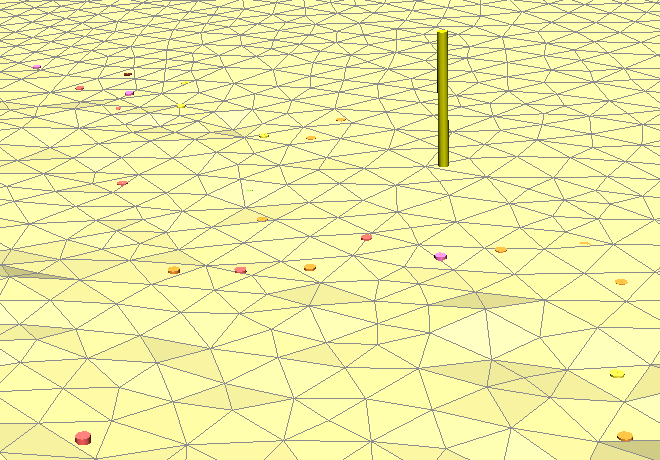
\includegraphics[width=0.48\linewidth]{error2}}
\end{center}
\caption{Examples for inconsistencies within the data. The left image show inconsistencies between two meshes. The right images show a number of boreholes, one of which has a wrong offset.} \label{fig:error}
\end{figure}

The render window is the part of the GUI where all the data is visualised in a user-controlled 3D scene. The process of ``drawing'' an object in the render window is technically called the \emph{rendering} of the object and will be referred to as such in the following. The render window is where you can actually see your data as well as the effects of all the changes you do somewhere else in the programm or in the input files.

One of the big advantages of the Data Explorer is in the fact that this visual inspection of the data also allows you to assess your data and to find inconsistencies and errors. Figure \ref{fig:error} gives examples of such inconsistencies.

You can manipulate the 3d view by using the mouse. Holding the left mouse button and moving the mouse rotation the view point around the focal point of the scene (by default this is the center point of your data). By holding the middle mouse button you can pan the view which means you translate left / right and up / down. By holding the right mouse button or moving the mouse wheel you can zoom in and out. There is alternative mouse button functionality assignment which is activated by holding the Spacebar. When activated left clicks pick a cell of the actually selected visualisation pipeline object. On right clicking the picked position is set as the focal point of the camera. This is useful for a better examination of an interesting region of the data so with focal point set to that region you can easily rotate and zoom around.

\subsection{Visualization Pipeline}

The visualisation pipeline looks very similar to the data views described above. However, the items displayed in this tab are a list of the graphical objects displayed (rendered) in the render window. For further reference these will be called \emph{visualisation items}. Each visualisation item has a checkbox beside its name that determines if the object is displayed in the render window or not. You can check or uncheck this box at any time, no data is lost if you uncheck it.

The relationship between data views, visualisation pipeline and render window is not completely straightforward without knowing the internal data structures of the programme but the basic concept is this:

For each data set loaded into the programme one or more visualisation items are created and then displayed in the render window. In most cases the relationship is not that difficult to understand: If a mesh is loaded, a new visualisation item is created and displayed in the render window. If a list of observation sites is loaded, again one visualisation item is created that represents the graphical object displayed in the render window. While you can expand that list of stations in the data view and see information about each station contained in the list, the visualisation item cannot be expanded. It is a substitute for the visualisation of said list in the render window. In the same vain, if a geometry is loaded into the programme up to \emph{three} visualisation objects are created: one for the list of points, one for the list of polylines and one for the list of surfaces (depending on the existence of polylines and surfaces).

Section \ref{filters} explains how you can employ the visualisation pipeline to apply filters the visualisation items. These filters allow changes of the way each object is visualised and they are quite handy to show certain aspects of the data.

\section{Writing Data...}

\subsection{Native Files}
You can save geometries, observation sites and meshes by right-clicking them in the Data View and selecting \cmd{Save data...}. You can also save all loaded data files by saving an \ogs project. Select \cmd{File\ra Save as...} and specify a project name. This option will save all geometries in *.gml files and all observation sites in *.stn files. Additionally it will create a project file (*.gsp). When loading the gsp-file later on it will also load the respective geometries and observation sites again.

\subsection{Export to Other Formats}

You can export data from \ogs into a number of graphics formats. This can be done for selected graphical objects by right-clicking the respective object in the visualisation pipeline and than select the desired format (VTK or OpenSG). Details on this can be found in section \ref{specvisoptions}.

You can also export the complete scene into the graphic formats VTK, OpenSG or VRML format. To do this select \cmd{File\ra Export\ra Format}. 